\chapter{Background and Related Work}\label{chap.background}
\minitoc
\section{Introduction}
At the heart of the \gls{ai} revolution lie neural networks, which are computational models inspired by the human brain. These algorithms have demonstrated an unprecedented ability to discern patterns, extract insights, and make predictions from vast amounts of data, often matching or even surpassing human capabilities in certain domains~\cite{silver2016mastering, gulshan2016development, lake2015human, xiong2016achieving, brown2020language}.

However, the explosive growth and complexity of neural networks have also given rise to significant computational challenges. Deep neural networks, characterized by their multi-layered architectures, can contain millions, if not billions, of parameters. Training and deploying these models demand elevated amounts of computational power. Traditional \gls{cpu}, while versatile, are not inherently optimized for the parallel and matrix-based computations that neural networks demand. This computational bottleneck not only impacts the speed and efficiency of neural network operations but also their energy consumption. This is a critical concern in our increasingly mobile and interconnected world.

Neural networks accelerators such as \glspl{gpu}, \glspl{tpu}, specialized \gls{asic}, and \gls{fpga}-based implementations have emerged as important players, providing the needed horsepower to drive neural computations swiftly and efficiently. As the quest for speed and efficiency continues, there is a growing interest in further refining these accelerators, particularly through custom numerical representations such as custom floating-point computation. This avenue promises a harmonious blend of performance and power efficiency, potentially announcing a new era for neural network engines.

This chapter examines the world of neural networks, starting with \glspl{snn} which mimic biological neuron behavior using time-sensitive spikes for communication. It then transitions into traditional \glspl{ann} to present the specifics of \glspl{cnn} that use continuous values. The discussion further explores their indelible mark on modern computation and the imperatives driving the development of dedicated hardware accelerators. Through this exploration, it is provided the background stage into low-power neural network accelerators leveraging custom floating-point computation a frontier at the nexus of \gls{ai} potential and practicality.

\section{Spiking Neural Networks}

\glspl{snn} offer an alternative paradigm in the neural computation landscape. Diverging from traditional \glspl{ann}, they emulate the temporal dynamics of biological neurons. Each neuron in an \gls{snn} accumulates input until a threshold is reached, upon which it emits a spike and resets. This behavior can be mathematically described by models such as the \gls{lif}~\cite{gerstner2014neuronal}:
\begin{equation}
\tau_m \frac{du(t)}{dt} = -u(t) + RI(t)
\end{equation}
where \( u(t) \) is the neuron membrane potential, \( \tau_m \) its time constant, \( R \) its resistance, and \( I(t) \) the input current. A spike is emitted when \( u(t) \) surpasses a threshold \( u_{\text{th}} \), followed by a reset.

Potential advantages of \glspl{snn} include energy efficiency, especially on neuromorphic hardware, and competence for processing temporal data~\cite{merolla2014million}. However, training \glspl{snn} presents challenges due to the non-differentiable nature of spikes~\cite{neftci2019surrogate}. Techniques range from gradient approximations for backpropagation~\cite{lee2016training}, surrogate gradient methods~\cite{neftci2019surrogate}, and unsupervised methods such as \gls{stdp}~\cite{masquelier2007unsupervised}.

\subsubsection{Spike-by-Spike Neural Networks} 

\label{sec:sbs}

\gls{sbs} is a spiking neural network based on a
generative probabilistic model. It iteratively finds an estimate of
its input probability distribution $p(s)$ (i.e. the probability of
input node $s$ to stochastically send a spike) by its latent variables
via $r(s) = \sum_i h(i) W(s|i)$, 
where $\vec{h}$ is an inference
population composed of a group of neurons that compete with each
other. An \gls{ip_sbs} sees only the spikes $s_t$ (i.e. the
index identifying the input neuron $s$ which generated that spike at
time $t$ produced by its input neurons, not the underlying input
probability distribution $p(s)$ itself. By counting the spikes
arriving at a group of \gls{sbs} neurons, $p(s)$ is estimated by
$\hat{p}(s) = 1/T \sum_t \delta_{s,s^t}$ after $T$ spikes have been
observed in total. The goal is to generate an internal representation
$r(s)$ from the string of incoming spikes $s_t$ such that the negative
logarithm of the likelihood
$L = C - \sum_\mu \sum_s \hat{p}_\mu(s) log\left( r_\mu(s) \right)$ is
minimized. $C$ is a constant which is independent of the internal
representation $r_\mu(s)$ and $\mu$ denotes one input pattern from an
ensemble of input patterns. Applying a multiplicative gradient descent
method on $L$, an algorithm for iteratively updating $h_\mu(i)$ with
every observed input spike $s_t$ could be derived
\cite{ernst2007efficient}:
\begin{eqnarray} \label{eq:sbs_update}
h_\mu^{new}(i) = \frac{1}{1+\epsilon} \left(h_\mu(i) + \epsilon \frac{h_\mu(i) W(s_t|i) }{\sum_j h_\mu(j) W(s_t|j)} \right) 
\end{eqnarray}
where $\epsilon$ is a parameter that also controls the strength of sparseness of the distribution of latent variables $h_\mu(i)$. Furthermore, $L$ can also be used to derive online and batch learning rules for optimizing the weights $W(s|i)$. The interested reader is referred to \cite{ernst2007efficient} for a more detailed exposition.

From a practical point of view, \gls{sbs} provides a mechanism to obtain a sparse representation of input patterns. Given a set of
training samples $\{x_\eta\}$, it learns weights ($W$), that allow
to express the input patterns as a linear sparse non-negative combination
of features.  During inference, it provides a mechanism for expressing
each test input $x_\mu$ as $x_\mu \approx W\, h_\mu$ where all
entries are non-negative.

The inference procedure consists in generating indices $s_t$
distributed according to a categorical distribution of the input pattern
$s_t \sim \mathrm{Categorical}(x_{\mu}(0), x_{\mu}(1), ..,
x_{\mu}(N-1))$. Starting with a random $h$ and executing
iteratively \Equ{eq:sbs_update} the \gls{sbs} algorithms finds
$h_{\mu}$. The fundamental concept of \gls{sbs} can be extended from vector to matrix
inputs. In this case, the linear operation $W\, h_\mu$ can be replaced by a
convolution to obtain a convolutional \gls{sbs} layer. A detailed description of the \gls{sbs} algorithm is presented in the Appendix~\ref{chap.append}

\paragraph{Basic Network Overview}

\gls{sbs} network models can be constructed in sequential layered structures \cite{rotermund2019Backpropagation}. Each layer consists of many \glspl{ip_sbs} (represented by $\vec{h}$), while the communication between them is organized by a low bandwidth signal -- the spikes.

The \gls{sbs} layer update is summarized in Algorithm~\ref{alg:sbs}. This is an iterative algorithm, where the number of spikes are denoted as ($N_{Spk}$), which is the number of iterations. As a generative model, each iteration updates the internal representation ($H$) based on the input spikes ($S^{in}_t$). A basic \gls{sbs} network architecture for handwritten digit classification (MNIST) is shown in \fig{fig:sbs_network} and \Tab{tab:sbs_network}. Each \gls{ip_sbs} is an independent computational entity, this allows to design specialized hardware architectures that can be massively parallelized (see \fig{fig:SbS_layer}).


\begin{algorithm}
	\caption{SbS layer update.}\label{alg:sbs}
	
	\begin{algorithmic}[1]
		\FOR {$t \leftarrow 0$ \textbf{to} $N_{Spk}-1$}
		\FOR {$x \leftarrow 0, y \leftarrow 0$ \textbf{to} $N_X-1, N_Y - 1$}
		\STATE $S^{out}_t(x, y) \sim Categorical( H^{}(x, y, :) ) $
		\FOR {$\Delta_X \leftarrow 0, \Delta_Y \leftarrow 0$ \textbf{to} $K_X - 1,K_Y - 1$}
		\STATE $spk \leftarrow S^{in}_t(x + \Delta_X , y + \Delta_Y)$
		\FOR {$i \leftarrow 0$ \textbf{to} $N_H-1$}
		\STATE $\Delta h(i)
		\leftarrow H^{}(x, y,  i) \cdot W^{}(\Delta_X, \Delta_Y, spk, i)$
		\STATE $r \leftarrow r + \Delta h(i)$
		\ENDFOR
		
		\FOR {$i \leftarrow 0$ \textbf{to} $N_H-1$}
		\STATE $H^{new}(x, y, i) \leftarrow \frac{1}{1+\epsilon} \left( H^{}(x, y, i) + \frac{\epsilon}{r} \Delta h(i) \right) $              
		\ENDFOR
		\ENDFOR
		\ENDFOR
		\ENDFOR
	\end{algorithmic} 
\end{algorithm}

\begin{figure*}
	\centering
	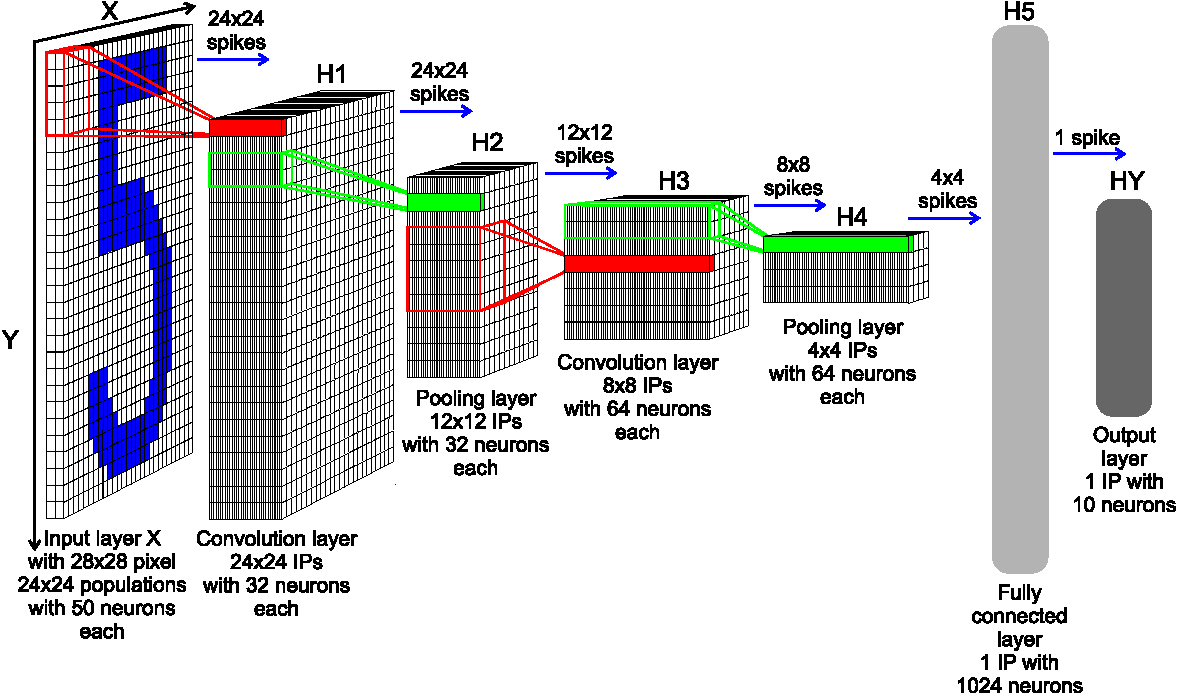
\includegraphics[width=0.5\columnwidth]{./chapters/sbs_accelerator/figures/sbs_network.pdf}
	\caption{\gls{sbs} network architecture for handwritten digit classification task.}
	\label{fig:sbs_network}
\end{figure*}


\begin{table}\centering
	\caption{\gls{sbs} network architecture for handwritten digit classification task.}
	\label{tab:sbs_network}
	\scriptsize
	\begin{tabular}{lrrrrrrr}\toprule
		&\multicolumn{3}{c}{\textbf{Layer size}} & &\multicolumn{2}{c}{\textbf{Kernel size}} \\\cmidrule{2-4}\cmidrule{6-7}
		\textbf{Layer} ($H^l$) &$N_X$ &$N_Y$ &$N_H$ & &$K_X$ &$K_Y$ \\\midrule
		Input ($HX$) &28 &28 &2 & &- &- \\
		Convolution ($H1$) &24 &24 &32 & &5 &5 \\
		Pooling ($H2$) &12 &12 &32 & &2 &2 \\
		Convolution ($H3$) &8 &8 &64 & &5 &5 \\
		Pooling ($H4$) &4 &4 &64 & &2 &2 \\
		Fully connected ($H5$) &1 &1 &1024 & &4 &4 \\
		Output ($HY$) &1 &1 &10 & &1 &1 \\
		\bottomrule
	\end{tabular}
\end{table}

\paragraph{Computational Cost}

The number of \gls{mac} operations required for inference of an \gls{sbs} layer is defined by $NOPS_{MAC}=N_{Spk} N_X N_Y K_X K_Y (3 N_H + 2)$, where $N_{Spk}$ is the number of spikes (iterations), $N_X N_Y$ is the size of the layer, $K_X K_Y$ is the size of the kernel for convolution/pooling, and $N_H$ is the length of $\vec{h}$. The computational cost of \gls{sbs} network models is higher compared to equivalent \gls{cnn} models and lower compared to regular \gls{snn} models (e.g., \gls{lif}) \mbox{\cite{izhikevich2004model}}.


\begin{figure*}
	\centering
	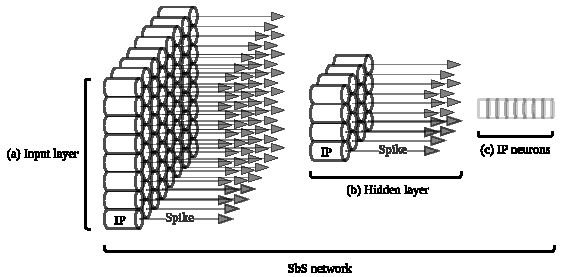
\includegraphics[width=0.5\columnwidth]{./chapters/sbs_accelerator/figures/SbS_layer.pdf}
	\caption{\gls{sbs} \glspl{ip_sbs} as independent computational entities, (a) illustrates an input layer with a massive amount of \glspl{ip_sbs} operating as independent computational entities, (b) shows a hidden layer with an arbitrary amount of \glspl{ip_sbs} as independent computational entities, (c) exhibits a set of neurons grouped in an \gls{ip_sbs}.}
	\label{fig:SbS_layer}
\end{figure*}


\paragraph{Error Tolerance}

To illustrate the error tolerance of \gls{sbs} networks, it is presented a classification performance under positive additive uniformly distributed noise as external disturbance. \fig{fig:robustnes_sbs} presents a comparison of the classification performance of an \gls{sbs} network and a standard \gls{cnn}, with the same amount of
neurons per layer as well as the same layer structure. Both neural networks are trained for handwritten digit classification on MNIST dataset \cite{lecun1998mnist} (see \cite{rotermund2019Backpropagation} for details). The figure shows the correctness for the MNIST test set with its \num[group-separator={,}]{10000} patterns in dependency of the noise level for positive additive
uniformly distributed noise. The blue curve shows the performance for
the \gls{cnn}, while the red curve shows the performance for
the \gls{sbs} network with \num[group-separator={,}]{1200} spikes (iterations). Beginning
with a noise level of 0.1, the respective performances are different
with a p - level of at least $10^{-6}$ (tested with the Fisher exact
test). Increasing the number of spikes per \gls{sbs} population to \num[group-separator={,}]{6000}
(performance values shown as black stars), shows that more spikes can
improve the performance under noise even more.

\begin{figure*}
	\centering
	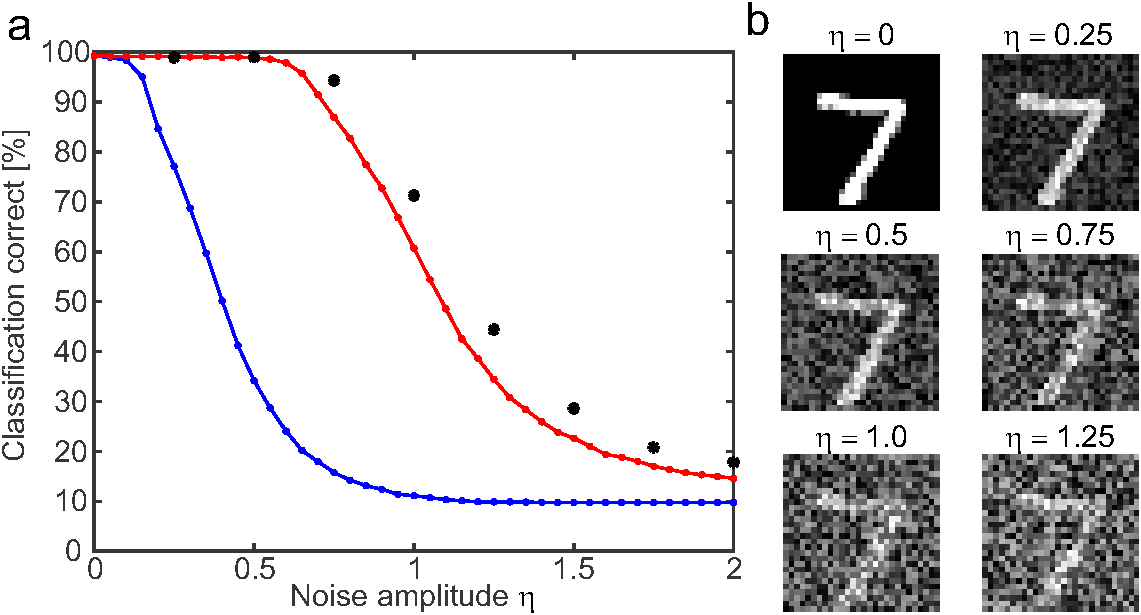
\includegraphics[width=0.5\columnwidth]{./chapters/sbs_accelerator/figures/sbs_robustnes.pdf}
	\caption{(a) Performance classification of \gls{sbs} NN versus equivalent \gls{cnn}, and (b) example of the first pattern in the MNIST test data set with different amounts of positive additive uniformly distributed noise.}
	\label{fig:robustnes_sbs}
\end{figure*}

\section{Artificial Neural Networks}
\glspl{ann} represent the main pillar in the \gls{ai}/\gls{ml} domain. Drawing inspiration from the networks of neurons in the human brain, \glspl{ann} have been designed to process information through interconnected nodes or "neurons". The concept of neural networks traces its roots back to the 1950s with the introduction of the perceptron by Frank Rosenblatt. The perceptron, a single-layer feedforward neural network, was among the first models capable of binary classifications~\cite{rosenblatt1958perceptron}. However, the limitations of perceptrons, including their inability to solve non-linearly separable functions, led to diminished interest in neural networks until the backpropagation algorithm emerged in the 1980s~\cite{rumelhart1986learning}. \glspl{ann} are designed to learn from data, allowing them to perform tasks without being explicitly programmed. Following this introduction, this section explores \glspl{ann}, with a particular focus on the specifics of \glspl{cnn}.

\subsection{Architecture}

Neural networks are computational models designed to extract patterns, interpret data, and approximate complex functions. Their architecture comprises interconnected nodes (neurons) organized into layers. Each connection possesses a weight value, which is adjusted during training. The primary components include:

\subsubsection{Layers}

\begin{itemize}
	\item \textbf{Input Layer}: Receives data. Given input data vector \( \mathbf{x} \) of dimension \( d \), the number of neurons is \( d \).
	\[
	\mathbf{x} = [x_1, x_2, ..., x_d]^\intercal
	\]
	
	\item \textbf{Hidden Layer(s)}: Transform the input using weighted connections. The output \( h \) of a neuron in a hidden layer is:
	\[
	h = f(\mathbf{w^\intercal} \cdot \mathbf{x} + b)
	\]
	where \( \mathbf{w} \) is the weights vector, \( b \) is a bias, and \( f \) is an activation function.
	
	\item \textbf{Output Layer}: Produces the predictions. The architecture depends on the task (e.g., regression, classification).
\end{itemize}

\subsubsection{Weights and Bias}

For each neuron, input data is transformed using weights and biases, adjusted during training. The weighted sum for a neuron is:
\[
z = \mathbf{w^\intercal} \cdot \mathbf{x} + b
\]

\subsubsection{Activation Functions}

Introduce non-linearities, enabling neural networks to capture complex relationships. Common functions include:

\begin{itemize}
	\item \textbf{Sigmoid}: 
The sigmoid function, denoted as \( \sigma(z) \), is especially used in binary decision tasks. Mathematically, the sigmoid function is defined as:

\[
\sigma(z) = \frac{1}{1 + e^{-z}}
\]

Here, \( z \) represents the input to the function. The function outputs a value between 0 and 1, making it especially useful for models where the output is a probability. 

The curve of the sigmoid function is S-shaped or sigmoidal. One of its properties is that its derivative (used in the backpropagation step of training neural networks) can be expressed in terms of the sigmoid function itself:

\[
\sigma'(z) = \sigma(z)(1 - \sigma(z))
\]

However, the sigmoid function is not without drawbacks. For very large or very small values of \( z \), the function becomes saturated, leading to small gradients and, consequently, slow convergence during training~\cite{glorot2010understanding}. This phenomenon is often referred to as the "vanishing gradient" problem.
	
	\item \textbf{Tanh}: 
The hyperbolic tangent function, denoted as \( \tanh(z) \), serves as an activation function in many neural network architectures. It scales and shifts the output of the sigmoid function to produce outputs in the range \([-1, 1]\). The mathematical expression for \( \tanh \) is:

\[
\tanh(z) = \frac{e^{z} - e^{-z}}{e^{z} + e^{-z}}
\]

Alternatively, it can be expressed in terms of the sigmoid function, \( \sigma(z) \), as:

\[
\tanh(z) = 2\sigma(2z) - 1
\]

The derivative of \( \tanh \), which is used during the backpropagation phase of neural network training, is given by:

\[
\frac{d}{dz}\tanh(z) = 1 - \tanh^2(z)
\]

Compared to the sigmoid function, \( \tanh \) is often preferred because its outputs are zero-centered, making it less likely to get stuck during training. However, it still suffers from the vanishing gradient problem for very large or very small values of \( z \).
	
	\item \textbf{ReLU}: 
The Rectified Linear Unit, commonly referred to as ReLU, has become one of the default activation functions, particularly for deep learning architectures. Mathematically, the ReLU function is defined as:

\[
f(z) = \max(0, z)
\]

In essence, the function returns \( z \) if \( z \) is greater than or equal to zero, and returns zero otherwise. This can be visualized as a linear function that will output the input directly if it is positive; otherwise, it will output zero.

The gradient of the ReLU function is binary:

\[
f'(z) = 
\begin{cases} 
1 & \text{if } z > 0 \\
0 & \text{otherwise}
\end{cases}
\]

One noted benefit of the ReLU function is its computational efficiency, given that it only requires a simple thresholding at zero. This allows models to train faster and requires less computational resources compared to other activation functions like sigmoid or tanh.

However, a potential drawback of the ReLU function is that units can sometimes get "stuck" during training and cease updating, leading to what's known as "dying ReLUs." The dying ReLU phenomenon can be viewed as a specific type of the vanishing gradient problem, where ReLU neurons become non-responsive and consistently output a value of zero, regardless of the input they receive. This is due to the fact that for inputs less than 0, the gradient is 0, which can cause weights to not update during backpropagation. To counteract this, variants like Leaky ReLU~\cite{maas2013rectifier} and Parametric ReLU~\cite{he2015delving} have been proposed.
\item \textbf{Softmax}:
In a neural network for multiclass classification tasks, the softmax function is a common choice for the activation function in the output layer. Given an input vector \( \mathbf{z} \) of length \( K \), representing the raw output (logits) of the \( K \) nodes in the output layer, the softmax function transforms these logits into a probability distribution over \( K \) classes. For each component \( i \) (where \( i = 1, 2, \ldots, K \)), the softmax function \( S(\mathbf{z}) \) is computed as:
\[
S(\mathbf{z})_i = \frac{{\exp(z_i)}}{{\sum_{j=1}^{K} \exp(z_j)}}
\]
where \( S(\mathbf{z})_i \) represents the \( i \)-th component of the output vector \( S(\mathbf{z}) \), \( \exp \) denotes the exponential function, and \( z_i \) is the \( i \)-th component of the input vector \( \mathbf{z} \). After applying the softmax function, each component of \( S(\mathbf{z}) \) is in the interval \( (0, 1) \), and the components sum to 1, allowing them to be interpreted as probabilities associated with each of the \( K \) classes. This makes the softmax function particularly useful for producing the final output in a neural network designed for classification tasks, as it ensures that the outputs are normalized and can be interpreted as class probabilities.

\end{itemize}

\subsection{Training Process}

Neural networks learn by adjusting weights and biases in response to training data. The goal is to minimize the difference between predictions and target values (the loss), often optimized using gradient-based methods.

\subsubsection{Stochastic Gradient Descent}

\gls{sgd} is an iterative optimization algorithm used to minimize an objective function that is defined as a sum of differentiable functions. This is particularly well-suited for problems with a large number of training samples~\cite{bottou2010large}.

Given an objective function \( J(\theta) \) which we aim to minimize, the objective is often defined as:
\[
J(\theta) = \frac{1}{N} \sum_{i=1}^{N} J_i(\theta)
\]
where \( J_i(\theta) \) is the loss associated with the \( i^{th} \) training example and \( \theta \) represents the parameters of the model.

The basic update rule for \gls{sgd} is:
\[
\theta \leftarrow \theta - \eta \nabla J_i(\theta)
\]
where:
\begin{itemize}
	\item \( \eta \) is the learning rate, a positive scalar determining the size of steps in the parameter space.
	\item \( \nabla J_i(\theta) \) is the gradient of the loss with respect to the parameters for the \( i^{th} \) training example.
\end{itemize}

In each iteration, a single training example \( (x_i, y_i) \) is picked randomly, and the model parameters are updated with the gradient of the loss \( J_i(\theta) \) with respect to that single example.

The iterative nature and use of only a single training example at each step make \gls{sgd} computationally more efficient compared to batch gradient descent, especially for large datasets~\cite{bottou2010large}. However, due to its stochastic nature, the trajectory of the parameters through the parameter space can be noisy, leading to a non-stable convergence to the minimum~\cite{bottou2018optimization}. Variants and improvements, like momentum~\cite{sutskever2013importance} or adaptive learning rates~\cite{duchi2011adaptive}, have been introduced to combat this instability and accelerate convergence.

\subsection{Multi-Layer Perceptron}

A \gls{mlp} is a type of feedforward artificial neural network, consisting of multiple layers of interconnected neurons~\cite{goodfellow2016deep}.

\subsubsection{Key Components}

\begin{itemize}
	\item An \textbf{input layer} that receives the data. The number of neurons in this layer corresponds to the dimensionality of the input data.
	
	\item One or more \textbf{hidden layers} that transform the input data. Each neuron in a hidden layer computes a weighted sum of its inputs, adds a bias term, and then applies an activation function.
	
	\item An \textbf{output layer} that provides the final prediction or classification results. The number of neurons in the output layer and their activation functions are tailored to the specific task.
\end{itemize}

Mathematically, the output \( o_{j} \) of the \( j^{th} \) neuron in any layer can be defined as:

\[
o_{j} = f\left( \sum_{i=1}^{N} w_{ij} x_{i} + b_{j} \right)
\]

where:
\begin{itemize}
	\item \( x_{i} \) is the output of the \( i^{th} \) neuron from the previous layer.
	\item \( w_{ij} \) is the weight associated with the connection between the \( i^{th} \) neuron from the previous layer and the \( j^{th} \) neuron of the current layer.
	\item \( b_{j} \) is the bias term for the \( j^{th} \) neuron.
	\item \( f \) is the activation function, which introduces non-linearity into the network.
\end{itemize}

The weights and biases of an \gls{mlp} are adjusted during the training phase.


\subsection{Convolutional Neural Networks}

\glspl{cnn} represent a specialized architecture in the deep learning domain, predominantly optimized for image and video processing tasks. Drawing inspiration from the human visual cortex structure and function, \glspl{cnn} are adept at automatically and adaptively discerning spatial hierarchies and patterns inherent in visual data~\cite{lecun1998gradient}.

\subsubsection{Key Components}

\begin{itemize}
	\item \textbf{Input Layer}: Responsible for ingesting raw pixel values from the image. The size is typically dictated by the resolution and depth (e.g., RGB channels) of the input.
	
	\item \textbf{Convolutional Layer}: At its core, the convolution operation involves sliding a filter over the input matrix to produce feature maps. Each filter aims to detect specific features, like edges or textures, in the input.
	
	\item \textbf{Activation Function}: Following the convolution operation, it is common to introduce non-linearity into the system. The ReLU is popularly employed in \glspl{cnn}.
	
	\item \textbf{Pooling Layer}: To reduce the spatial dimensions and computational load, the pooling layer down-samples feature maps. Max pooling is a widely adopted strategy:
	\begin{equation}
	Z = \max(W ^ X)
	\end{equation}
	where \(W\) is the window applied to the input matrix \(X\).
	
	\item \textbf{Fully Connected Layer}: This layer sees each neuron connected to every activation from the previous layer, effectively acting as a standard multi-layer perceptron. It linearizes the features extracted from preceding layers and approximates a function, which commonly is an image classification or regression task.
	
	\item \textbf{Output Layer}: Generates the final class scores, typically in a probabilistic form via a softmax function.
\end{itemize}

A relevant characteristic of \glspl{cnn} is weight sharing, this substantially reduces the number of parameters, thus diminishing the risk of overfitting. Through their capacity to hierarchically discern two-dimensional patterns, \glspl{cnn} have been relevant in furthering advancements in a variety of fields, spanning from sensor analytics to medical image analysis and autonomous vehicle vision systems.

\subsubsection{Conv2D Tensor Operation}
A convolutional layer aims to learn and extract feature representations from a given input. Each unit of a feature map is connected to a region of neighboring units on the input maps (from the previous layer). This neighborhood in the previous layer is known as the receptive field of such unit. A new feature map can be obtained by first convolving the input maps with a learned kernel and then applying a nonlinear elementwise activation function to the convolved results. All spatial locations on the input maps share a kernel to generate a feature map. All feature maps are obtained by convolving several different kernels~\cite{gu2018recent}.


The 2D convolution process is performed by the \emph{Conv2D} tensor operation, described in \Equ{eq:conv2D}, where $W$ is the convolution kernels (known as filters), $b$ is the bias vector for the output feature maps, and $h$ is the input tensor containing the feature maps~\cite{goodfellow2016deep}. $K\times L\times M$ is the receptive field size, $K\times L$ is the convolution kernel, and $M$ is the number of input channels/feature maps. Mathematically, the \emph{Conv2D} operator is defined as:
\begin{eqnarray} \label{eq:conv2D}
Conv2D\left(W,b,h\right)_{i,j,o}=\sum_{k,l,m}^{K,L,M} h_{(i+k,j+l,m)} W_{(o,k,l,m)}+b_{o}
\end{eqnarray}

\subsubsection{Computational Cost of a Convolution Layer}

The computational complexity of a convolution layer primarily depends on the spatial dimensions of the input and the kernel, the number of input and output channels, and the stride (slide step) with which the kernel is applied. For clarity, a list of definitions and concepts is presented:

\paragraph{Definitions}
\begin{itemize}
	\item \( W_i \): Width of the input feature map.
	\item \( H_i \): Height of the input feature map.
	\item \( D_i \): Depth (number of channels) of the input feature map.
	\item \( W_k \): Width of the kernel.
	\item \( H_k \): Height of the kernel.
	\item \( D_k \): Depth of the kernel. Typically, \( D_k = D_i \).
	\item \( N_o \): Number of output feature maps (number of kernels in the layer).
	\item \( S \): Stride of the convolution.
\end{itemize}

\paragraph{Computations Per Output Element}

For each kernel position on the input feature map, the number of multiply and accumulate operations is defined by:
\begin{equation}
2 \times W_k \times H_k \times D_k
\end{equation}

\paragraph{Output Dimensions}

Given the stride \( S \), the dimensions of the output feature map are:
\begin{align}
W_o &= \frac{W_i - W_k}{S} + 1 \\
H_o &= \frac{H_i - H_k}{S} + 1
\end{align}

\paragraph{Total Computations}

For each output feature map, the total operations are:
\begin{equation}
W_o \times H_o \times 2 \times W_k \times H_k \times D_k
\end{equation}

Given \( N_o \) output feature maps, the entire convolution layer's computational cost becomes:
\begin{equation}
N_o \times W_o \times H_o \times 2 \times W_k \times H_k \times D_k
\end{equation}

This represents the number of multiply-accumulate operations in a convolution layer. Other considerations might include biases and employed activation functions, but the above calculation primarily signifies the computational burden of the convolution operation.

\subsubsection{Error Tolerance in Convolution Layers}

Deep neural networks, especially \glspl{cnn}, have exhibited an advantageous property: they possess a significant degree of robustness to various perturbations in their computations, including reduced-precision arithmetic and the introduction of noise. This error tolerance characteristic of convolution layers has paved the way for various optimization techniques aiming to reduce the computational and storage overhead without sacrificing too much in performance~\cite{han2015deep}.

\paragraph{Sources of Error}

Errors in convolution layers can arise from various sources:
\begin{itemize}
	\item \textbf{Quantization:} Converting \gls{fp} precision weights and activations to a lower bit-width representation.
	\item \textbf{Pruning:} Setting certain weights to zero to reduce the total number of weights.
	\item \textbf{Approximate Computing:} Techniques that purposefully introduce computational errors by simplifying compute hardware to improve power efficiency, area, and speed.
\end{itemize}

\paragraph{Error Compensating Mechanisms}

There are several hypotheses and mechanisms that explain the error tolerance:

\begin{itemize}
	\item \textbf{Overparameterization:} Many deep models have more parameters than necessary for the task. This data redundancy can help the network adapt to small errors.
	\item \textbf{Re-training:} After introducing errors (like in quantization), the network can be fine-tuned to recover some of the lost performance.
	\item \textbf{Regularization Effect:} Some error introduction techniques, like quantization, can act as a form of regularization, potentially helping to prevent overfitting.
\end{itemize}

\paragraph{Exploiting Error Tolerance for Optimization}

Leveraging the error resilience of convolution layers can lead to several benefits:

\begin{itemize}
	\item \textbf{Reduced Precision:} Weights and activations can be represented with fewer bits, leading to a reduced memory footprint and computation savings.
	\item \textbf{Energy Efficiency:} Approximate computing techniques can yield significant power savings.
	\item \textbf{Faster Computations:} Reduced precision arithmetic can be faster and allows for parallelism.
\end{itemize}

Understanding and harnessing the error tolerance properties of convolution layers present opportunities for designing more efficient and compact neural network implementations, especially vital for low-power devices and real-time applications. While errors can be introduced to an extent, it remains crucial to ensure that the network accuracy does not degrade beyond acceptable levels.


\section{Neural Network Accelerators}
Neural network accelerators are specialized hardware components or platforms designed to accelerate the computationally intensive tasks associated with neural networks. Their primary goal is to enhance performance, reduce power consumption, and provide real-time processing capabilities for \gls{ai}/\gls{ml} applications~\cite{sze2017efficient}.

\subsection{The Need for Accelerators}
Neural networks come with intensive computational and memory demands due to their deep architectures and vast numbers of parameters:

\begin{itemize}
	\item \textbf{Compute Cost}: \gls{ai}/\gls{ml} models, especially \glspl{cnn} and transformers, are characterized by their deep architectures. Each layer involves a large number of weights and activations. In the forward pass (inference), for each neuron, the input activations are multiplied by corresponding weights, and then all these products are accumulated to produce the neuron output. Similarly, during training, the backpropagation algorithm is also computation-costly.
	
	\item \textbf{Memory Cost}: \gls{ai}/\gls{ml} models, especially those with millions or even billions of parameters, require elevated memory footprint for model storage. During computation, the frequent access to weights, along with the need to read and write intermediate activations, can stress the memory bandwidth. Memory access is also energy-expensive, often more than the actual arithmetic operations.
	
	As illustration, the memory requirements for an \gls{mlp} are:
	\begin{enumerate}
		\item \textbf{Weights Storage}: Given a deep neural network with \(L\) layers, where each layer \(l\) has \(n_l\) neurons and receives input from \(n_{l-1}\) neurons, the number of weights (excluding biases) is:
		\begin{align*}
		W &= \sum_{l=2}^{L} n_l \times n_{l-1}
		\end{align*}
		
		\item \textbf{Activations Storage}: Activations need to be stored for the forward pass and are particularly crucial during training for the backpropagation process. For a given layer \(l\), activations storage requirement is proportional to \(n_l\), and the total for the entire network is:
		\begin{align*}
		A &= \sum_{l=1}^{L} n_l
		\end{align*}
	\end{enumerate}
	Considering both weights and activations, the memory access pattern becomes a bottleneck, especially when the model size exceeds the on-chip memory capacity, leading to frequent off-chip accesses which are both time and energy-consuming.
	
	\item \textbf{Real-time Requirements}:
	Many contemporary applications demand instantaneous or near-instantaneous processing due to their interactive or safety-critical nature. Hence, the computational backend supporting such applications, often driven by deep neural networks, must be optimized for low-latency and high-throughput to meet the real-time requirements.
	
	\item \textbf{Energy Efficiency}: Many modern devices, from smartphones to \gls{iot} sensors, operate on limited power sources such as batteries. For these devices, the power-hungry computations of \gls{ai}/\gls{ml} models can quickly drain the battery, limiting usability, applicability, and functionality. Given that neural network computations are becoming pervasive, even in these power-constrained devices, energy efficiency is of vital importance.
	
	The proliferation of \gls{ai}/\gls{ml} applications in low-power devices imposes strict constraints on energy consumption. Factors driving this need include:
	
	\begin{enumerate}
		\item \textbf{Battery Capacity}: Most low-power devices rely on battery power. High energy consumption due to intensive computations can drastically reduce operational time between charges, affecting applicability.
		
		\item \textbf{Form Factor and Heat Dissipation}: Smaller devices have smaller batteries and reduced space for cooling mechanisms, making them susceptible to overheating. Hence, energy-efficient computations are not only about battery longevity but also about device temperature, safety, and size.
		
		\item \textbf{Operational Continuity in Low-Power Devices}: Many edge devices, such as sensors, are expected to operate continuously. These devices might be located in hard-to-reach places, making frequent battery replacements impractical. Thus, energy efficiency is crucial for operational viability and application feasibility.
	\end{enumerate}
	
\end{itemize}

Given these challenges, it is needed to optimize neural network deployments on such devices at both software and hardware levels to achieve desired performance within the power constraints.

\subsection{Types of Accelerators}

In the dynamic landscape of \gls{ai}/\gls{ai}, various hardware accelerators, including \glspl{gpu}, \glspl{asic}, \glspl{fpga}, and \glspl{npu}, have emerged to optimize and facilitate neural network computations.
\begin{itemize}
	\item \textbf{\glspl{gpu}}: Historically designed for the purpose of graphics rendering, \glspl{gpu} have architecture that naturally perform parallel computing. This parallelism is especially beneficial for neural network computations involving repetitive and simultaneous operations. As a result, \glspl{gpu} have become a cornerstone for deep learning training and inference.
	
	The success of \glspl{gpu} in the \gls{ai}/\gls{ml} domain is evident from the rise of \gls{gpu}-optimized deep learning frameworks and the continuous evolution of \gls{gpu} architectures tailored for neural network computations.
	
	
	\item \textbf{\glspl{asic}}: they can provide significant benefits in terms of power, performance, and area over general-purpose processors. One of the most notable \glspl{asic} designed for neural network computations is Google's \gls{tpu}. Neuromorphic chips, like IBM's TrueNorth or Intel's Loihi, are \glspl{asic} designed to mimic the synapse-neuron connections in the human brain, potentially offering more efficient ways to handle neural network tasks, especially for real-time processing and low-power scenarios.
	
	\item \textbf{\glspl{fpga}}: \glspl{fpga} represent a bridge between general-purpose processors and \glspl{asic} in terms of adaptability and performance:
	
	\begin{enumerate}
		\item \textbf{Reconfigurability}: Unlike \glspl{asic}, which are fixed in their functionality post-manufacture, \glspl{fpga} can be reprogrammed to adopt different logic functions. This means they can be tailored to accelerate specific neural network operations and then reconfigured for another task if needed.
		
		\item \textbf{Parallelism}: \glspl{fpga} excel in parallel processing, with their array of logic blocks and interconnects. Neural network computations, which often involve concurrent operations on data, can be accelerated by exploiting this parallelism.
		
		\item \textbf{Prototyping and Evolution}: Given their reconfigurable nature, \glspl{fpga} are excellent platforms for prototyping neural network architectures. Furthermore, in environments where neural network models evolve or get updated frequently, \glspl{fpga} can adapt without requiring new hardware.
		
		\item \textbf{Trade-offs}: While \glspl{fpga} offer flexibility, they might not achieve the same level of performance or energy efficiency as a highly-optimized \gls{asic} for a specific task. However, their adaptability can outweigh this in certain scenarios.
	\end{enumerate}
	
	In the context of the rapidly evolving field of \gls{ai}/\gls{ml}, \glspl{fpga} provide a compelling balance of adaptability and performance, especially when agility in hardware is desired.
	
	\item \textbf{\glspl{npu}}: \glspl{npu} are dedicated hardware accelerators optimized for neural network computation. \glspl{npu} streamline both training and inference processes by focusing on operations and data flow patterns typically found in neural networks, resulting in enhanced energy efficiency and performance compared to general-purpose processors.
	
\end{itemize}

\subsection{Design Considerations}
For neural network accelerator design, it is important to address key considerations such as precision, memory hierarchy, scalability, and flexibility, each of which plays a crucial role in ensuring optimal performance and adaptability in the evolving \gls{ai}/\gls{ml} domain.

\begin{itemize}
	\item \textbf{Precision}: In neural network accelerator design, the precision of arithmetic operations plays a pivotal role. Employing reduced precision arithmetic offers dual advantages: it can markedly accelerate computations and simultaneously diminish power consumption. However, it is crucial to preserve a balance to ensure that the reduced precision does not compromise the accuracy and reliability of the neural network model.
	
	\item \textbf{Memory Hierarchy and Dataflow}: Memory hierarchy and dataflow are tightly coupled in the design of efficient neural network accelerators. Dataflow refers to the way data is passed and processed between different memory hierarchies and computation units. The choice of dataflow can dramatically impact the energy efficiency, latency, and throughput of the accelerator.
	
	For neural networks, especially deep learning models, the memory access pattern plays a significant role in determining overall performance. This is because fetching data (e.g., weights, activations) from memory often consumes more energy and time than the arithmetic computations themselves.
	\item \textbf{Scalability}: The capability of a neural network accelerator to extend its computational capacity to handle larger neural networks or to elevate existing hardware performance. This extension can be achieved by either increasing the resources within a single chip (vertical scaling) or by distributing the computation across multiple chips or processing units (horizontal scaling).
	
	As neural network models become more complex and demand more computational resources, it is crucial for accelerators to be scalable. This ensures that they can continue to provide accelerated performance for newer and larger models without requiring a complete redesign.
	A modular approach facilitates easy addition of processing units or modules to address scalability needs.
	\item \textbf{Flexibility}: Flexibility remains a cornerstone in the design of neural network accelerators. While tailoring hardware for specific tasks or models can yield substantial performance boosts, it is imperative that these accelerators retain the versatility to accommodate a diverse range of neural network models and operations. This ensures a balance between optimized performance and broad applicability, allowing for both efficiency and adaptability in ever-evolving \gls{ai}/\gls{ml} landscapes.
	
\end{itemize}

\section{Precision and Effect in Training}

Conventional neural networks typically rely on regular \gls{fp} arithmetic. However, to optimize computational speed, minimize memory footprint, and reduce energy consumption, hardware accelerators adopt lower precision formats. While this can speed up operations and reduce resource demands, there is a trade-off as reduced precision might affect the model accuracy. Therefore, balancing precision and performance is crucial, with techniques such as mixed-precision and dynamic/custom arithmetic being employed to navigate these trade-offs~\cite{micikevicius2017mixed}.
\subsection{Fixed-Point}

Fixed-point arithmetic represents numbers with a fixed number of digits before and after the decimal point, in contrast to floating-point where the decimal point can "float". Leveraging fixed-point arithmetic offers distinct advantages. Specifically, fixed-point operations are more resource-efficient, leading to expedited computations. Additionally, their inherent simplicity in arithmetic operations often translates to diminished power consumption. 


However, while fixed-point arithmetic offers efficiencies in many neural network applications, there are situations where it may not be ideal:

\begin{enumerate}
	\item \textbf{Training}: During training, the need to represent small weight updates and gradient values is critical. \gls{fp} arithmetic is often preferred to ensure effective backpropagation, whereas fixed-point might impede convergence or acceptable model accuracy~\cite{courbariaux2014training}.
	
	\item \textbf{High-Precision}: For tasks requiring acute precision, such as medical imaging or anomaly detection, fixed-point arithmetic might compromise prediction accuracy, especially when using fewer bits.
	
	\item \textbf{Transfer Learning and Fine-Tuning}: In scenarios such as fine-tuning pre-trained models, small gradient values are crucial. The reduced precision of fixed-point might neglect these subtle updates.
	
	\item \textbf{Normalizing and Batch Normalization}: Operations involving a diverse range of values, like normalization, might introduce significant quantization errors when using fixed-point representations~\cite{jacob2018quantization}.
	
	\item \textbf{\glspl{rnn}}: \glspl{rnn}, due to their sequential nature and sensitivity to numerical precision, can experience issues such as exploding or vanishing gradients with fixed-point arithmetic.
	
	\item \textbf{Activation Functions with Exponential Ranges}: Functions such as softmax, which operate over a wide range, might be susceptible to quantization errors in a fixed-point context.
\end{enumerate}

While quantization techniques continue to evolve, it remains essential to rigorously evaluate fixed-point representations in the above contexts to ensure desired performance and accuracy.



\subsection{Floating-Point}
\gls{fp} arithmetic offers distinct advantages due to its capability to represent numbers with both high precision and a wide dynamic range. However, while it provides granular accuracy, it typically demands more computational resources and power compared to fixed-point arithmetic. The inherent robustness of neural networks to numerical perturbations implies a potential avenue for exploring custom reduced-precision \gls{fp} arithmetic.

The representation of every numerical value, in any numerical system, is made of an integer and a fractional part. The border that delimits them is called the radix point. The fixed-point format for representing numeric values derives its name from the fact that in this format, the base point is fixed at a certain position. For integer numbers, this position is at the right of the least significant digit.

In scientific computation, it is often necessary to represent very large and very small values. This is difficult to achieve using the fixed-point format because the bit size required to maintain both the desired precision and the desired range are very large. In such situations, \gls{fp} formats are used to represent real numbers. Each \gls{fp} number can be divided into three fields: sign $S$, exponent $E$, and mantissa $M$. Using the binary number system, it is possible to represent any \gls{fp} number as:

\begin{eqnarray} \label{eq:float}
(-1)^{S} \times 1.M \times 2^{E-B}
\end{eqnarray}

In \gls{fp} representations the exponent is biased. This bias depends on the bit size of the exponent field. This exponent bias is defined by \Equ{eq:float_bias}, where $E_{size}$ is the exponent bit size.

\begin{eqnarray} \label{eq:float_bias}
B=2^{E_{size}-1}-1
\end{eqnarray}

There is a natural trade-off between small bit size requiring fewer hardware resources and larger bit size providing higher precision. Within a given total bit size, it is possible to assign various combinations of sizes to the exponent and mantissa fields, with wider exponents resulting in a higher range and wider mantissa resulting in better precision.

The most widely used format for \gls{fp} arithmetic is the IEEE 754 standard \cite{zuras2008ieee}. The IEEE single-precision format (32-bit) is expressed by \Equ{eq:float} with $B$ = 127, 8 bits for the exponent and 23 bits for the mantissa, see \Fig{fig:floating}(a). In \gls{fp} formats, the numbers are normalized, the leading one is an implicit bit, and only the fractional part is explicitly stored in the mantissa field.

\begin{figure*}
	\centering
	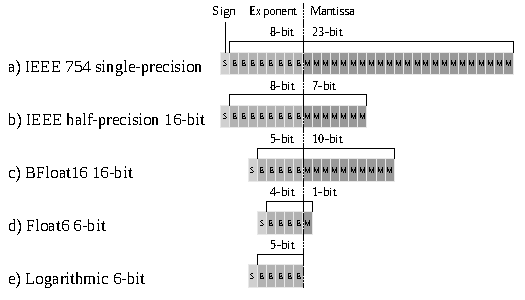
\includegraphics[width=0.5\columnwidth]{./chapters/cnn_accelerator/figures/power_breakdown/floating_point.pdf}
	\caption{Floating-point number representation.}
	\label{fig:floating}
\end{figure*}

Reduced bit size than those specified in the IEEE 754 standard are often sufficient to provide the desired precision. Reduced designs require fewer hardware resources enabling low-power implementations. In custom hardware designs, it is possible to customize the \gls{fp} format implemented. In later sections, the term E$a$M$b$ is used to denote \gls{fp} formats, where $a$ and $b$ are the exponent and mantissa bit size, respectively. For example, E4M1 means 4-bit exponent and 1-bit mantissa, see \Fig{fig:floating}(d).

There are three special definitions in IEEE 754 standard. The first is subnormal numbers when $E=0$, then \Equ{eq:float} is modified to \Equ{eq:float_subnorm}. Infinity and \gls{nan} are the other two special cases but are not used in our work.

\begin{eqnarray} \label{eq:float_subnorm}
(-1)^{S} \times 0.M \times 2^{1-B}
\end{eqnarray}

Transitioning a neural network model from high-precision to lower-precision computations presents a set of challenges. One of the most critical of these challenges lies in preserving the accuracy of the model while it operates under conditions of reduced numerical precision. This balance requires thoughtful consideration and strategic implementation to ensure that the benefits of computational efficiency do not come at the cost of significant degradation in model performance.

\subsection{Post-Training Quantization}

In \gls{ptq}, a neural network, once fully trained, undergoes a conversion process wherein its \gls{fp} weights and activations are mapped to a lower precision~\cite{krishnamoorthi2018quantizing}.

Given the full precision weights \( W \) of a neural network, they can be quantized to a lower precision using the quantization function:
\begin{equation}
Q(W) = \text{round}\left(\frac{W}{\Delta}\right) \times \Delta
\end{equation}
where \( \Delta \) is a quantization step size, often derived from the range of the weights or activations and the target precision.

One challenge of \gls{ptq} is to ensure minimal loss of accuracy after the conversion. Techniques such as fine-tuning the quantized model, applying regularization during initial training, or using advanced quantization schemes (e.g., mixed precision) can aid in preserving the model accuracy.

While \gls{ptq} offers the benefit of simplicity, the resultant quantized model might not be as robust or accurate as models trained with \gls{qat} techniques. However, for many applications, especially those on resource-constrained devices, the slight trade-off in accuracy is often outweighed by the benefits in computational efficiency, memory usage, and power consumption.


\subsection{Quantization-Aware Training}

\gls{qat} is a technique developed to optimize neural networks for deployment on platforms with limited numerical precision. This quantization maps weights to a lower precision \( Q(W) \), similarly as in \gls{ptq}. Moreover, \gls{qat} integrates this process into the training phase, ensuring that the resultant model is resilient to potential accuracy degradation~\cite{krishnamoorthi2018quantizing}. Such adaptations are relevant when targeting resource-constrained devices or specialized hardware accelerators that rely on reduced precision for improved computational efficiency and accuracy.

For neural networks with custom reduced \gls{fp} formats, \gls{qat} exhibits even greater versatility. Such custom formats, often denoted as \( FP_{M,E} \), allocate specific bit-lengths for the mantissa \( M \) and the exponent \( E \). The function for this quantization format is detailed in \Algo{alg:quantizr}. This algorithm converts full-precision values into their corresponding quantized \gls{fp} representation using custom-defined exponent and mantissa bit lengths.

\begin{algorithm}[h!]
	\caption{Custom floating-point quantizer.}
	\label{alg:quantizr}
	\begin{algorithmic}
		\SetAlgoLined
		\renewcommand{\algorithmicrequire}{\textbf{input:}}
		\renewcommand{\algorithmicensure}{\textbf{output:}}
		\REQUIRE $X_{FP}$ as the \gls{fp} value.
		\REQUIRE $E_{size}$ as the target exponent bit size.
		\REQUIRE $M_{size}$ as the target mantissa bits size.
		\REQUIRE $STDM_{size}$ as the IEEE 754 mantissa bit size.
		\ENSURE $X_{CFP}$ as the custom \gls{fp} value.
		
		\STATE $sign \gets GetSign(X_{FP})$
		\STATE $exp \gets GetExponent(X_{FP})$
		\STATE $fullexp \gets 2^{E_{size}-1}-1$ // Get full range value
		\STATE $cman \gets GetCustomMantissa(X_{FP}, M_{size})$
		\STATE $leftman \gets GetLeftoverMantissa(X_{FP}, M_{size})$
		\IF {$exp <-fullexp$}
		\STATE$X_{CFP}\gets0$
		\ELSIF{$exp > fullexp$}
		\STATE$X_{CFP}\gets (-1)^{sign}\cdot2^{fullexp}\cdot(1+(1-2^{-M{size}}))$
		\ELSE
		\IF {$2^{STDM_{size}-M_{size}-1}-1<leftman$}
		\STATE $cman \gets cman+1$ // Above halfway
		\IF{$2^{M_{size}}-1<cman$}
		\STATE $cman \gets 0$ // Correct mantissa overflow
		\STATE $exp \gets exp + 1$
		\ENDIF
		\ENDIF
		\STATE // Build custom \gls{fp} representation
		\STATE$X_{CFP}\gets (-1)^{sign}\cdot2^{exp}\cdot(1+cman\cdot2^{-M_{size}})$
		\ENDIF
	\end{algorithmic}
\end{algorithm}

During training, each forward pass applies the aforementioned quantization, simulating the operational conditions of the reduced precision. The backward pass, essential for gradient-based optimization, is conducted with a higher precision. If \( \nabla W \) symbolizes the computed gradients, the weight update rule in gradient descent is typically:
\begin{equation}
W_{t+1} = W_t - \eta \nabla W
\end{equation}
Here, \( \eta \) represents the learning rate. However, with \gls{qat}, the model remains cognizant of \( Q(W) \) or \( Q_{FP}(W) \) during forward computations, a factor that influences gradient dynamics. Post-\gls{qat}, calibration using a validation dataset aids in refining scaling factors or biases, this improves the model for optimal performance in its intended deployment environment. Assessments against a full-precision baseline are important to ensure that the trade-offs in precision do not compromise the model efficacy.

\section{Dataflow Taxonomy}
Dataflow taxonomy refers to the classification of various schemes that determine how data (weights, activations, and partial results) moves through the accelerator during computation. The way data is moved and reused can have an impact on the energy efficiency and throughput of the accelerator. These strategies aim to maximize performance and energy efficiency by optimizing data movement, which is often more energy-intensive than computation itself. When choosing or designing a dataflow, it is essential to consider the specific neural network workload, the memory hierarchy, and the architectural details of the hardware to ensure an optimal match~\cite{sze2017efficient}.

\subsection*{Weight Stationary (WS)}
In this dataflow, weights are kept stationary in the processing elements. As different input activations come in, they are multiplied with these stationary weights. This approach maximizes the reuse of weights, which can be beneficial when processing a large number of activations, such as during a convolution operation.
Characteristics:
\begin{align*}
\textbf{Fixed:} & \quad \text{Weights} \\
\textbf{Moving:} & \quad \text{Activations, Partial Sums}
\end{align*}

\subsection*{Output Stationary (OS)}
Here, the partial results (output activations) are kept stationary. Weights and input activations move through the processing elements and the partial sums are accumulated in place. This scheme tries to maximize the reuse of the output from the computation, which is beneficial when a given output is the result of multiple accumulations. Characteristics:
\begin{align*}
\textbf{Fixed:} & \quad \text{Partial Sums} \\
\textbf{Moving:} & \quad \text{Weights, Activations}
\end{align*}

\subsection*{Input Stationary (IS)}
In this scheme, input activations remain stationary, while weights move through and are multiplied with these stationary activations. This can be beneficial when a single activation is used in multiple computations. Characteristics:
\begin{align*}
\textbf{Fixed:} & \quad \text{Activations} \\
\textbf{Moving:} & \quad \text{Weights, Partial Sums}
\end{align*}

\subsection*{No Local Reuse (NLR)}
As the name suggests, in this dataflow, there is minimal local data reuse. All data types-weights, activations, and partial sums-move through the processing elements. This is often not as efficient in terms of energy consumption since there is a lack of reuse; however, it is simpler in terms of control and design. Characteristic:
\begin{align*}
\textbf{Moving:} & \quad \text{Weights, Activations, Partial Sums}
\end{align*}

\subsection*{Row Stationary (RS)}
This is a specialized dataflow developed for systolic array architectures. In RS, a row of the systolic array holds the activations stationary while weights are propagated horizontally and partial sums propagate vertically.


\section{Flynn's Taxonomy}

In the quest to comprehend the various computational architectures, especially when focusing on neural network accelerators and their efficiency, it is important to grasp the foundational classification of computer architectures. Flynn's Taxonomy, introduced by Michael J. Flynn in 1966, provides a categorical breakdown of architectures based on their simultaneous instruction and data streams handling capability.

\subsection*{SISD (Single Instruction, Single Data)}

This category represents the classic sequential computer architecture, where a single instruction operates on a single data stream. Most conventional \glspl{cpu} can be categorized here, though modern designs often include multiple cores (making them multiprocessors).

\subsection*{SIMD (Single Instruction, Multiple Data)}

Under \gls{simd}, a single instruction processes multiple data streams concurrently. This design is prevalent in vector processors and \glspl{gpu}. Given the parallel nature of neural network computations, \gls{simd} architectures, particularly \glspl{gpu}, have gained popularity for deep learning and neural network tasks due to their ability to process multiple data points in parallel using the same operation.

\subsection*{MISD (Multiple Instruction, Single Data)}

This architecture is less common and represent systems where multiple instructions operate on a single data stream. Some fault-tolerant machines adopt this strategy, applying different operations to replicate the data to ensure reliability.

\subsection*{MIMD (Multiple Instruction, Multiple Data)}

These systems are where multiple processors operate independently on different instructions and different data. Multi-core \glspl{cpu}, clusters, and many supercomputers belong to this category. Each processor can be assigned a unique task, making them suitable for a broader range of applications compared to \gls{simd}.

\subsection*{Relevance to Neural Network Accelerators}

When discussing low-power neural network accelerators with custom reduced \gls{fp} computation, \gls{simd} architectures often stand out. The parallel nature of neural networks leverages the capabilities of \gls{simd} to handle multiple data points concurrently.

\section{Multiply-Accumulate Unit}

In the context of this dissertation, the terms 'dot-product' and '\gls{mac}' are used interchangeably, reflecting their deeply associated roles in computational processes. The dot-product, a pivotal operation in neural network computation, entails a sequence of multiplications culminating in a summation. This procedure aligns seamlessly with the series of \gls{mac} operations, a cornerstone in the field of digital signal processing. The \gls{mac} operation, with its inherent structure and efficiency, stands as a central pillar in the architecture and optimization of neural network accelerators. Formally, the \gls{mac} operation can be expressed as:
\begin{equation}
\text{ACC} = \text{ACC} + (A \times B)
\end{equation}
Where:
\begin{itemize}
	\item \( \text{ACC} \): Represents an accumulator accumulating the results of the products.
	\item \( A \) and \( B \): Operands subjected to multiplication.
\end{itemize}

In neural computations, a substantial number of \gls{mac} operations are executed. To elucidate, consider the convolutional layer in a \gls{cnn}. This layer predominantly requires \gls{mac} operations to compute the weighted sum of inputs and respective weights. If we denote \( x[i] \) as a data array or vector of input values and \( w[i] \) as the weights, an output \( y \) for a specified filter and input position can be delineated as:
\begin{equation}
y = \sum_{i} x[i] \cdot w[i]
\end{equation}
This summation is fundamentally a sequence of \gls{mac} operations.

\subsection{Design Considerations}
Several considerations come into play to ensure optimal performance, efficiency, and versatility of \gls{mac} hardware modules.

\begin{enumerate}
	\item \textbf{Computational Efficiency}: Contemporary neural network models, particularly those under the deep learning paradigm, necessitate executing billions of \gls{mac} operations. An well engineered hardware \gls{mac} unit can amplify the computation speed. The number of clock cycles it takes to complete a \gls{mac} operation can impact the overall performance. High performance is often achieved using parallelism techniques, pipelining, and array-based hardware architectures.
	
	\item \textbf{Power Dynamics}: The magnitude of \gls{mac} operations in neural networks means that even marginal inefficiencies can escalate into significant power consumption. A carefully designed \gls{mac} unit, potentially integrating advanced techniques such as quantization or approximation, can mitigate power exigencies.
	
	\item \textbf{Precision Dynamics}: Neural networks, in certain architectures, can accommodate reduced precision. However, the essence of a dynamic \gls{mac} unit design is to navigate the balance between computational efficiency and precision.
	
	\item \textbf{Scalability Factors}: The ever-evolving domain of neural networks is marked by models growing in complexity and depth. A \gls{mac} unit, based on modular design principles, can be seamlessly scaled across extensive accelerator architectures, serving to the spectrum of models.
	
	\item \textbf{Adaptive Flexibility}: The dynamism inherent in neural network architectures necessitates a \gls{mac} unit enriched with the capacity to adapt to diverse operations, varied data typologies (e.g., floating-point, fixed-point), and a range of hybrid/custom precisions.
\end{enumerate}

The \gls{mac} operation holds a pivotal role in the field of neural network accelerator design. The \gls{mac} design directly influences the accelerator performance, power efficiency, and overall effectiveness.



\section{Related Work}
For efficient neural network computation, two main optimization strategies are used, namely network compression and classical approximate computing~\cite{bouvier2019spiking}. Researchers focusing on low-power embedded applications started lowering the precision of weights and activation maps to compress the memory footprint of the large number of parameters representing \glspl{ann}, a method known as network compression or quantization. This practice takes advantage of the intrinsic error-tolerance of neural networks, as well as their ability to compensate for approximation while training. In this way, reduced bit precision causes a small accuracy loss~\cite{courbariaux2015binaryconnect, han2015deep, hubara2017quantized, rastegari2016xnor}.


In addition to quantization, network pruning reduces the model size by removing structural portions of the parameters and its associated computations~\cite{lecun1989optimal,hassibi1992second}. This method has been identified as an effective technique to improve the efficiency of \gls{dnn} for applications with limited computational budget~\cite{molchanov2016pruning,li2016pruning, liu2018rethinking}.


\subsection{Aggressive Quantization}
In hardware development, \gls{wq} has shown up to $2\times$ improvement in energy consumption with an accuracy degradation of less than $1\%$ \cite{moons20160, whatmough201714}. Some advanced quantization methods yield to \glspl{bnn} allowing the use of \glspl{xnor} instead of the conventional costly \glspl{mac}~\cite{rastegari2016xnor}. In~\cite{sun2018xnor}, Sun \textit{et al.} report an accuracy of $98.43\%$ on handwritten digit classification (MNIST) with a simple \gls{bnn}. Hence, quantization is a powerful tool for improving the energy efficiency and memory requirements of \gls{ann} accelerators, with limited accuracy degradation.

\subsection{Spiking Neural Network Accelerators}

These methods can be used for \glspl{snn} as well. In~\cite{rathi2018stdp}, Rathi \textit{et al.} report up to $3.1\times$ improvement in energy consumption with an accuracy loss of around $3\%$. Weight quantization allows the designer to realize a trade-off between the accuracy of the \gls{snn} application and efficiency of resources. Approximate computing can also be applied at the neuron level, where irrelevant units are deactivated to reduce the computation cost of the \glspl{snn}~\cite{sen2017approximate}. This computation skipping can be applied randomly on synapses, training \glspl{ann} with stochastic synapses improves generalization, resulting in a better accuracy~\cite{srivastava2014dropout, wan2013regularization}. Such methods are compatible with \glspl{snn} and have been tested both during training~\cite{neftci2016stochastic, srinivasan2016magnetic} and operation \cite{buesing2011neural}, and even to define the connectivity between layers \cite{bellec2017deep, chen20184096}. Implementations of spiking neuromorphic systems in \gls{fpga}~\cite{sheik2016synaptic} and hardware~\cite{jerry2017ultra} demonstrated that synaptic stochasticity allows to increase the final accuracy of the networks while reducing memory footprint.

Quantization is therefore a powerful technique to improve energy efficiency and memory requirements of \gls{ann} and \gls{snn} accelerators, with small accuracy degradation. However, this approach requires \gls{qat} methods that, in some cases, are problematic or even inaccessible, particularly in emerging deep \gls{snn} algorithms~\cite{zhang2018survey}.

\subsubsection{Classical Approximate Computing}
Approximate computing has been used in a wide range of applications to increase the computational efficiency in hardware~\cite{han2013approximate}. This approach consists of designing processing elements that approximate their computation by employing modified algorithmic logic units~\cite{han2013approximate}. In~\cite{kim2013energy}, Kim \textit{et al.} have shown \glspl{snn} using carry skip adders achieving $2.4\times$ latency enhancement and $43\%$ more energy efficiency, with an accuracy degradation of 0.97\% on a handwritten digit classification task (MNIST). Therefore, approximate computing provides important enhancement in energy efficiency and processing speed.

However, as the complexity of the dataset increases, as well as the depth of the network topology, such as ResNet~\cite{he2016deep} on ImageNet~\cite{russakovsky2015imagenet}, the accuracy degradation becomes more important and may not be negligible anymore~\cite{rastegari2016xnor}, especially for critical applications such as autonomous driving. Therefore, it is not certain that network compression techniques and approximate computing are suitable for all applications.

\subsubsection{Spike-by-Spike Neural Network Accelerators}
Rotermund \textit{et al.} demonstrated the feasibility of a neuromorphic \gls{sbs} \gls{ip_sbs} on a Xilinx Virtex 6 \gls{fpga}~\cite{rotermund2018massively}. It provides a massively parallel architecture, optimized to reduce memory access and suitable for \gls{asic} implementations. Nonetheless, this design is considerably resource-demanding if implemented as a full \gls{sbs} network in today's embedded technology.

\subsection{Convolutional Neural Network Accelerators with Custom Floating-Point Computation on \gls{fpga}
}
\label{sec:related_work}
In the literature we find plenty of hardware architectures for \gls{cnn} accelerators implemented in \gls{fpga}. Most of the research work implements fixed-point quantization, and very limited research focuses on \gls{fp}. Moreover, to the best of my knowledge, there is no research work related to \gls{fp} inference for low-power embedded applications.


\subsubsection{Hybrid Custom Floating-Point}
In \cite{lai2017deep}, Liangzhen Lai \textit{et al.} proposed a mixed data representation with floating-point for weights and fixed-point for activations. This work demonstrated on SqueezeNet, AlexNet, GoogLeNet, and VGG-16 that 8-bit floating-point quantization (4-bit exponent and 3-bit mantissa) results in constant negligible accuracy degradation. Similarly, in \cite{settle2018quantizing}, Sean O. Settle \textit{et al.} presented an 8-bit \gls{fp} quantization scheme, which needs an extra inference batch to compensate for quantization errors. However, \cite{lai2017deep} and \cite{settle2018quantizing} did not present a dedicated hardware architecture.

In \cite{lian2019high}, Xiaocong Lian \textit{et al.} proposed a hardware accelerator with optimized block floating-point (BFP). In this design the activations and weights are represented by 16-bit and 8-bit \gls{fp} formats, respectively. This design is demonstrated on Xilinx VC709 evaluation board. This implementation achieves throughput and power efficiency of \unit[760.83]{GOP/s} and \unit[82.88]{GOP/s/W}, respectively. However, this design is not suitable for low-power resource-constrained embedded \glspl{fpga}.

\begin{figure}[h!]
	\centering
	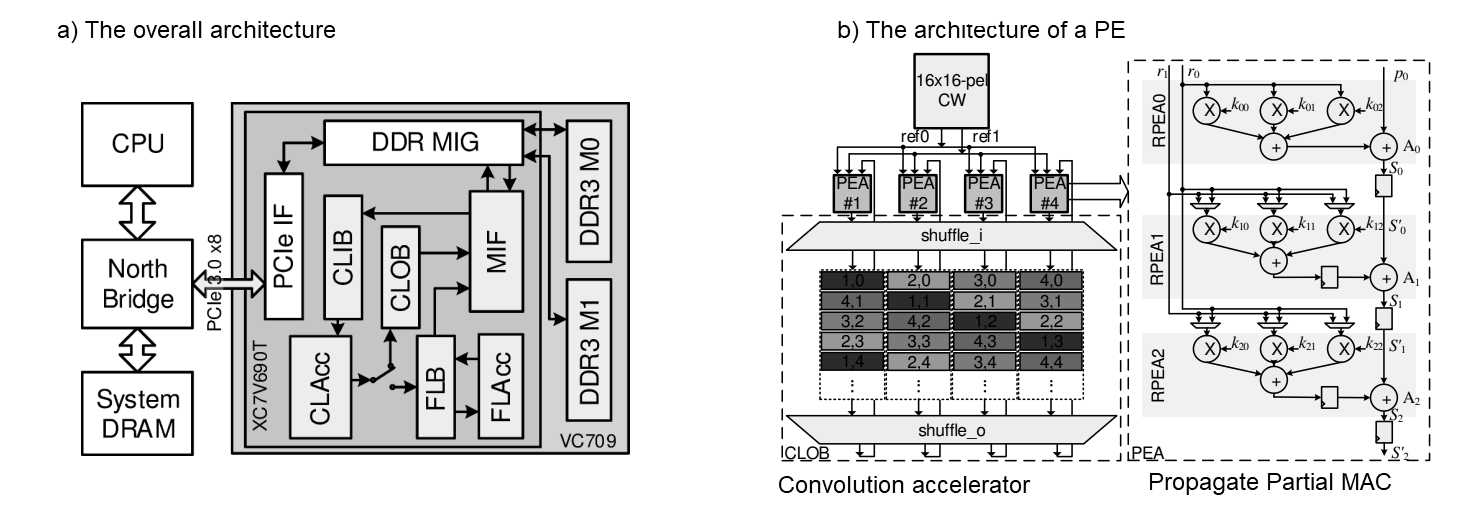
\includegraphics[width=\textwidth]{./figures/1_g.png}
	\caption{1.}
	\label{fig:1}
\end{figure}
\FloatBarrier

\subsubsection{Low-Precision Floating-Point}
In \cite{mei2017200mhz}, Chunsheng Mei \textit{et al.} presented a hardware accelerator for VGG16 model using half-precision \gls{fp} (16-bit). This design is demonstrated on Xilinx Virtex-7 (XC7VX690T) with PCIe interface. This implementation achieves throughput and power efficiency of \unit[202.8]{GFLOP/s} and \unit[18.72]{GFLOP/s/W}, respectively. In \cite{wu2021low}, Chen Wu \textit{et al.} proposed a low-precision (8-bit) floating-point (LPFP) quantization method for \gls{fpga}-based acceleration. This design is demonstrated on Xilinx Kintex 7 and Ultrascale/Ultrascale+. This implementation achieves throughput and power efficiency of \unit[1086.8]{GOP/s} and \unit[115.4]{GOP/s/W}, respectively. While these studies concentrate on low-precision \gls{fp}, they are not optimal for inference on low-power devices due to their size, power consumption, and cost.

\begin{figure}[h!]
	\centering
	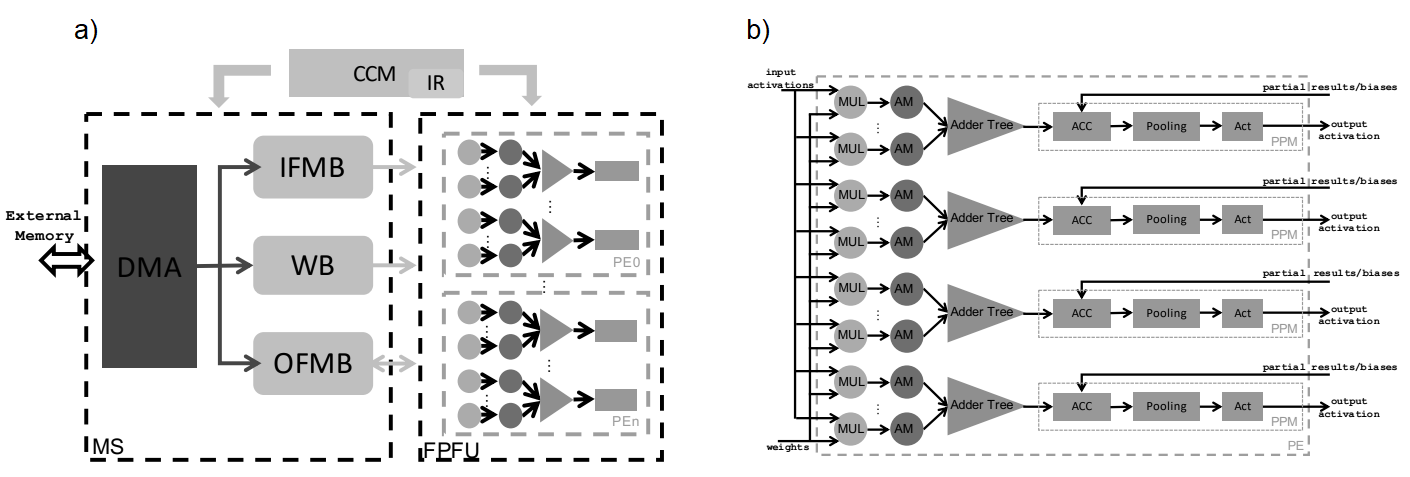
\includegraphics[width=\textwidth]{./figures/2_g.png}
	\caption{2.}
	\label{fig:2}
\end{figure}

\begin{figure}[h!]
	\centering
	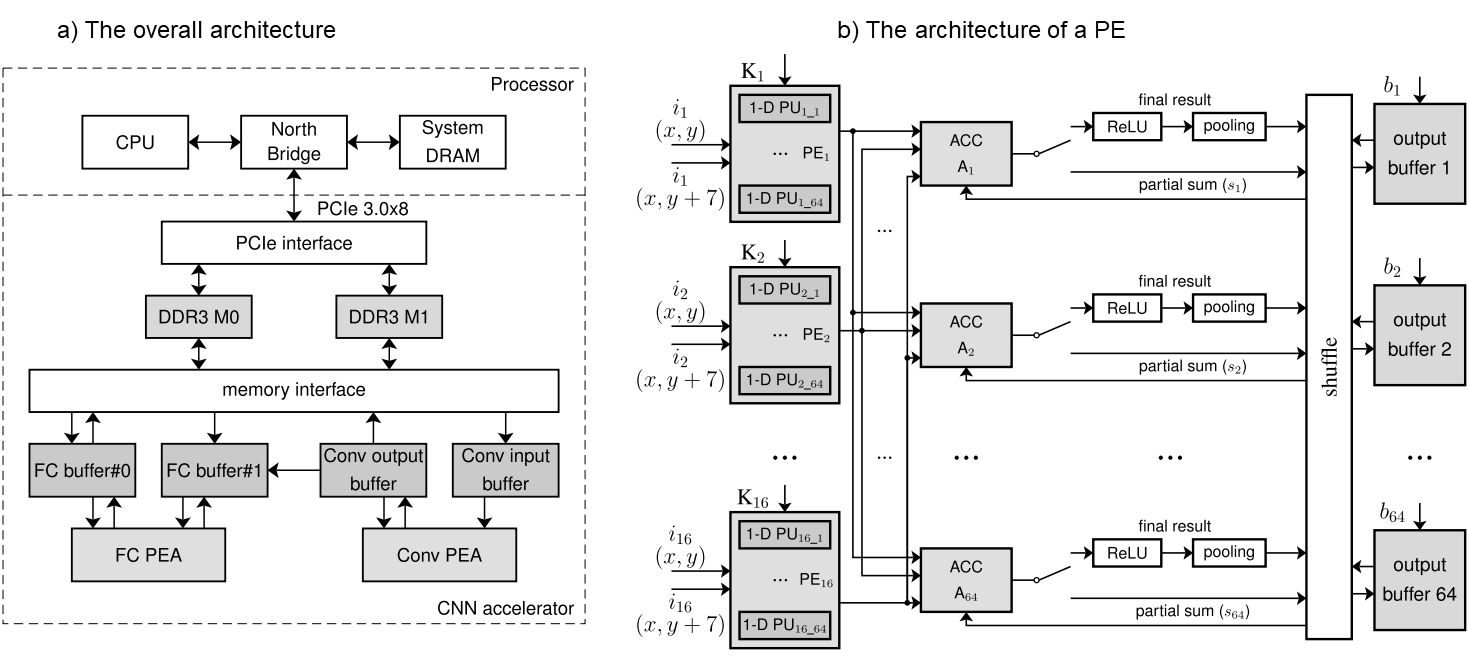
\includegraphics[width=\textwidth]{./figures/3_g.png}
	\caption{3.}
	\label{fig:3}
\end{figure}
\FloatBarrier

\subsubsection{Low-Power Architectures for \gls{iot} Deployments}
Two research papers have showcased hardware accelerator designs for the XC7Z007S, the most resource-constrained and low-power device in the Zynq-7000 \gls{soc} \gls{fpga} series. Its development board, MiniZed, is priced at USD 89.00. This device serves as the central target of this dissertation for low-power \gls{cnn} acceleration.

In \cite{meloni2019cnn}, Paolo Meloni \textit{et al.} presented a \gls{cnn} inference accelerator for compact and cost-optimized devices. However, this implementation uses fixed-point to process light-weight \gls{cnn} architectures with a power efficiency between \unit[2.49] to \unit[2.98]{GOPS/s/W}.

\begin{figure}[h!]
	\centering
	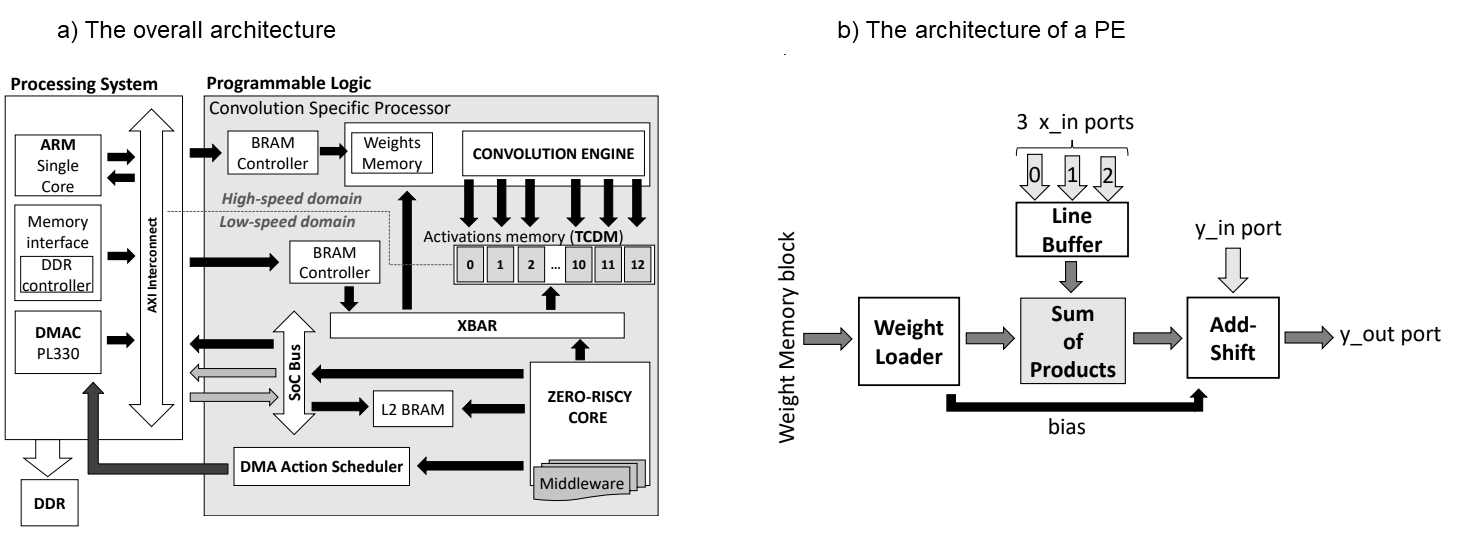
\includegraphics[width=\textwidth]{./figures/4_g.png}
	\caption{4.}
	\label{fig:4}
\end{figure}
\FloatBarrier

In \cite{gao2020edgedrnn}, Chang Gao \textit{et al.} presented EdgeDRNN, a \gls{rnn} accelerator for edge inference. This implementation adopts the \gls{snn} inspired delta network algorithm to exploit temporal sparsity in \glspl{rnn}. However, this implementation does not include \gls{fp} computation.
%%%%%%%%%%%%%%%%%%%%%%%%


\subsection{Neural Network Accelerators for Training and Inference with 8-bit Floating-Point Computation on \gls{asic}
}
State-of-the-art low-power neural network accelerators have demonstrated significant improvements in both energy efficiency and computational performance using 8-bit \gls{fp} arithmetic for training and inference. The studies presented in this subsection uniformly explore the advantages of 8-bit \gls{fp} quantization, specifically with a composition of a 4-bit exponent and 3-bit mantissa for high-accuracy inference, and a 5-bit exponent with a 2-bit mantissa for training.

\cite{wu2020phoenix} proposes the Phoenix architecture implementing 8-bit \gls{fp} quantization. Key findings suggest that this method incurs less error than its fixed-point counterpart. Normalization prior to quantization aids in further error reduction (less than 0.5\% for top-1 and 0.3\%
for top-5 accuracy degradation). Phoenix outperforms other state-of-the-art accelerators when benchmarked with AlexNet and VGG16. The circuit placement and routing results show that Phoenix achieves peak performance of \unit[2.048]{TMAC/s} with \unit[1.44]{mm$^2$} and \unit[1091.2]{mW} at TSMC \unit[28]{nm} technology, respectively. Compared with a state-of-the-art accelerator, Phoenix achieves 3.32$\times$ and 7.45$\times$ better performance with
the same core area for AlexNet and VGG-16, respectively.
Compared with Nvidia TITAN Xp \gls{gpu}, Phoenix consumes
151$\times$ less energy with single image inference.

Another work, \cite{park2021neural}, presents an 8-bit \gls{fp} neural network training processor that leverages shared exponent bias (FP8-SEB) for non-sparse neural networks. This implementation uses multiple-way fused multiply-add (FMA) trees for maintaining high numerical precision and reducing energy consumption, demonstrating improved efficiency against conventional neural network training processors. Fabricated in \unit[40]{nm} LP CMOS, the processor consumes
\unit[13.1]{mW} at \unit[0.75]{V}, \unit[20]{MHz} with the maximum energy efficiency of \unit[4.81]{TFLOPS/W}, and \unit[230]{mW} at \unit[1.1]{V}, \unit[180]{MHz} with the maximum performance of \unit[567]{GFLOPS} and area efficiency of \unit[90.7]{GFLOPS/mm$^2$}   .

\cite{venkataramani2021rapid} introduces a 4-core \gls{ai} chip, called RaPiD, an accelerator that supports various precisions. Notably, the accelerator can handle 16 and 8-bit \gls{fp} computations, as well as 4 and 2-bit fixed-point calculations. Measurements show INT4 inference for batch size of 1 yields 3 - 13.5 (average 7) TOPS/W and FP8 training for a mini-batch of 512 achieves a sustained 102 - 588 (average 203) TFLOPS across a wide range of applications.

Lastly, \cite{venkataramanaiah202228nm} discusses an 8-bit \gls{fp} tensor core-based CNN training processor. This processor incorporates highly parallel tensor cores, ensuring high utilization throughout various phases of the training process. With the integration of dynamic output activation sparsity and other efficiency-enhancing features, this 28nm prototype chip showcases energy efficiency of \unit[16.4]{TFLOPS/W}.



\subsection{Training Techniques with 8-bit Floating-Point Quantization}
In the continued pursuit of refining neural network training, the application of 8-bit \gls{fp} quantization -- employing a 5-bit exponent with 2-bit mantissa for training, and a 4-bit exponent with 3-bit mantissa for inference -- has risen as a common key strategy, as demonstrated by the subsequent studies.

One of the early explorations into this field was the use of 8-bit \gls{fp} for training the LeNeT-5 model for handwritten digit classification, achieving a commendable 97.10\% accuracy (2\% degradation) while reducing space complexity by 75\% \cite{gallus2018handwritten}. A similar work demonstrated the feasibility of training, for the first time, deep neural networks using 8-bit \gls{fp} numbers, introducing novel techniques such as chunk-based accumulation and \gls{fp} stochastic rounding, which holds the potential for up to 4 times improved throughput in future hardware platforms \cite{wang2018training}.

A significant milestone is the hybrid 8-bit \gls{fp} (HFP8) format, which was specifically crafted for deep learning applications ranging from image classification to language processing -- AlexNet, ResNet, MobileNetV2, DenseNet121, LSTMs, Transformer, MaskRCNN, and SSD-Lite -- trained on datasets like ImageNet, PennTreeBank, WMT14 En-De, SWB300, COCO, and VOC, highlighting minimal accuracy degradations when transitioning from baseline FP32 to Hybrid FP8 training. \cite{sun2019hybrid}. This was further optimized in a mixed precision training approach that utilized an enhanced loss scaling method and a stochastic rounding technique to address gradient noise, reporting even better accuracies than full precision across multiple data sets (imagenet-1K, WMT16) and a broader set of workloads (Resnet-18/34/50, GNMT, Transformer) \cite{mellempudi2019mixed}.

Taking a different approach, adaptive floating-point (AFP) post-training quantization emerged as a promising approach, offering compression rates and inference efficiency, avoiding the need for computationally intensive \gls{qat}, this work presents a framework to automatically optimize and choose the adequate AFP configuration for each layer, thus maximizing the compression efficacy. This approach demonstrates that AFP-encoded ResNet-50/MobileNet-v2 only has 0.04/0.6\% accuracy degradation wrt its full-precision counterpart \cite{liu2021improving}.

In conclusion, 8-bit floating-point quantization emerges as a pivotal strategy, echoing the industry need for efficiency, compactness, and precision in neural network training.
